
\section{講義概要}


\begin{frame}
\frametitle{今日の内容}



\begin{enumerate}
\item 二変数関数, 極限, 連続性
\item 偏微分, 高次偏導関数,
\item 接平面, 極値問題, ヘッセ行列式
\end{enumerate} 



\end{frame}
\begin{slide}{二変数関数のグラフの書き方(excel編)}

二次元のテーブルを作成(例:twodim.xlsx)して、グラフから3-D等高線を選択。
\begin{figure}[h]
\centering
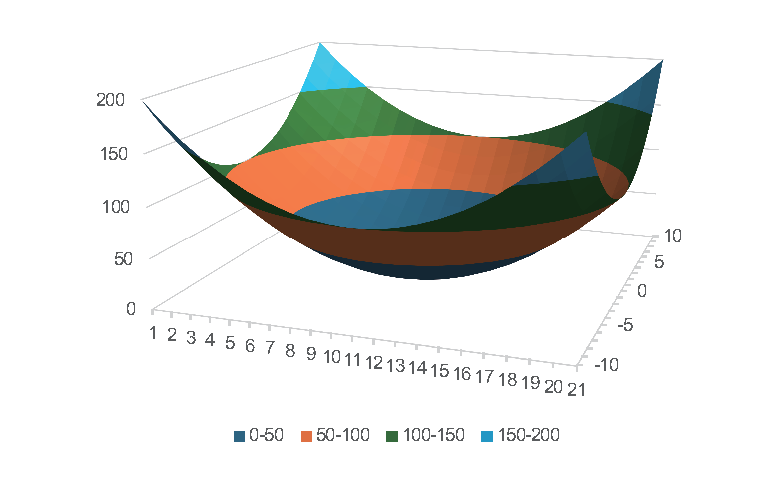
\includegraphics[width=8cm]{calculus10/twodim.eps}
\end{figure}
簡単に書けるが、グラフの向きを変更するには角度などを投入する必要があり、直観的でない。

\end{slide}
\begin{frame}[fragile]
\frametitle{二変数関数のグラフの書き方(MATLAB編)}
以下のようにプログラム(m scriptと呼ばれる)。

 \begin{lstlisting}
x = (-10:1:10);
y = (-10:1:10);
f = zeros(21,21);
for i=1:21
    for j=1:21
          f(i,j) = x(i)*x(i)+y(j)*y(j);
    end
end
surf(x,y,f);
 \end{lstlisting}
\begin{figure}[h]
\centering
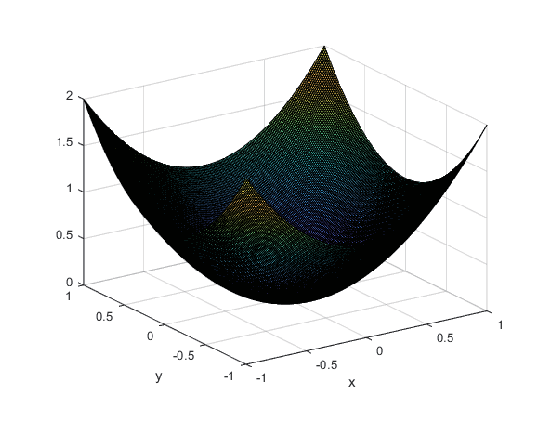
\includegraphics[width=5cm]{calculus10/twodimmatlab.eps}
\end{figure}

\end{frame}




%%%%%%%%%%%%%%%%%%%%%%%%%%%%%%%%%%%%%%%%%%%%%%%%%%%%%%%%%%%%%%%%%%%%%%%%%%%%%%%%%%%%%%%
%%%%%%%%%%%%%%%%%%%%%%%%%%%%%%%%%%%%%%%%%%%%%%%%%%%%%%%%%%%%%%%%%%%%%%%%%%%%%%%%%%%%%%%


%%%%%%%%%%%%%%%%%%%%%%%%%%%%%%%%%%%%%%%%%%%%%%%%%%%%%%%%%%%%%%%%%%%%%%%%%%%%%%%%%%%%%%%
%%%%%%%%%%%%%%%%%%%%%%%%%%%%%%%%%%%%%%%%%%%%%%%%%%%%%%%%%%%%%%%%%%%%%%%%%%%%%%%%%%%%%%%



\section{二変数関数}


\begin{frame}
\frametitle{二変数関数}


これまでは一変数関数を議論してきたが, 今回は二変数関数を考える. 
%より一般の二変数関数の理論は二変数関数の理論と同様なので


\begin{Def}
部分集合$D \subset \R^2$に対して, 写像$f:D\rightarrow \R$を\underline{二変数関数}という. 
$x,y$を$\R^2$の標準的な座標として, $f(x,y)$などと書かれる場合が多い. 
\end{Def}

\begin{itemize}
\item $f(x,y)=2x^3-xy^2+y^2+3$. 定義域は$\R^2$. 
\item $g(x,y)=\sqrt{5-2x^2-y^2}$. 定義域は楕円板$\{2x^2+y^2 \le 5\}$. 

\end{itemize}


\end{frame}



%%%%%%%%%%%%%%%%%%%%%%%%%%%%%%%%%%%%%%%%%%%%%%%%%%%%%%%%%%%%%%%%%%%%%%%%%%%%%%%%%%%%%%%
%%%%%%%%%%%%%%%%%%%%%%%%%%%%%%%%%%%%%%%%%%%%%%%%%%%%%%%%%%%%%%%%%%%%%%%%%%%%%%%%%%%%%%%



\section{二変数関数}


\begin{frame}
\frametitle{二変数関数のグラフ}


$xyz$-空間$\R^3$上の点$(x,y,f(x,y))$を考えることで, 関数$f(x,y)$を可視化できる. 
集合
$$
\{(x,y,f(x,y)) \ | \ (x, y) \in D\} \subset \R^3
$$
を関数$f(x,y)$の\underline{グラフ}という. 

\vspace{-3mm}

\begin{figure}[htbp]
 \begin{center} 
  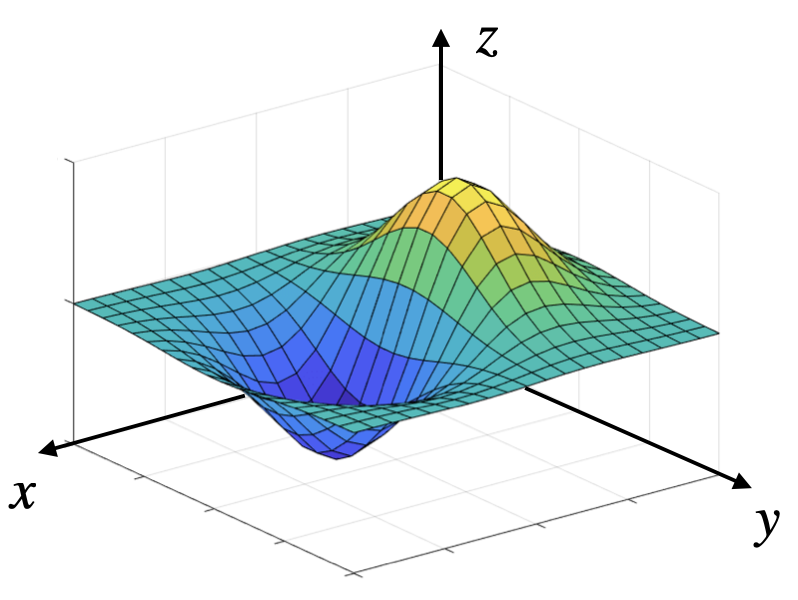
\includegraphics[width=55mm]{calculus10/graph3d.png}
 \end{center}
\end{figure}

\vspace{-3mm}

\end{frame}




%%%%%%%%%%%%%%%%%%%%%%%%%%%%%%%%%%%%%%%%%%%%%%%%%%%%%%%%%%%%%%%%%%%%%%%%%%%%%%%%%%%%%%%
%%%%%%%%%%%%%%%%%%%%%%%%%%%%%%%%%%%%%%%%%%%%%%%%%%%%%%%%%%%%%%%%%%%%%%%%%%%%%%%%%%%%%%%

\section{極限}


\begin{frame}
\frametitle{距離}

極限を定義するために, まず2点間の距離を定義する

\begin{Def}
$\R^2$上の$2$点$(x,y)$と$(a,b)$の\underline{距離}を次で定義. 
$$
\mathrm{d}((x,y),(a,b))=\sqrt{(x-a)^2+(y-b)^2}. 
$$
\end{Def}

\vspace{-2mm}

\begin{figure}[htbp]
 \begin{center} 
  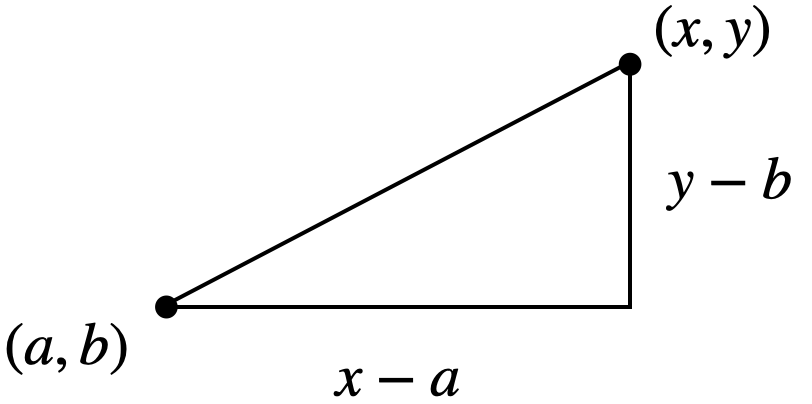
\includegraphics[width=40mm]{calculus10/dist.png}
 \end{center}
\end{figure}

\vspace{-2mm}

\end{frame}


%%%%%%%%%%%%%%%%%%%%%%%%%%%%%%%%%%%%%%%%%%%%%%%%%%%%%%%%%%%%%%%%%%%%%%%%%%%%%%%%%%%%%%%
%%%%%%%%%%%%%%%%%%%%%%%%%%%%%%%%%%%%%%%%%%%%%%%%%%%%%%%%%%%%%%%%%%%%%%%%%%%%%%%%%%%%%%%


\begin{frame}
\frametitle{極限}


\begin{Def} \label{極限}
\begin{itemize}
\item $(x,y) \to (a,b)$を$\mathrm{d}((x,y),(a,b)) \to 0$として定義. 
\item $(x,y) \to (a,b)$なるとき, 
 \begin{itemize}
 \item $f(x,y)\to \alpha \in \R$であることを
$$
\lim_{(x,y)\to (a,b)}f(x,y)=\alpha, 
$$
\item  $f(x,y)$の値がいくらでも大きく(小さく)なることを
$$
\lim_{(x,y)\to (a,b)}f(x,y)=+ \infty \ (-\infty)
$$
\end{itemize}
と書く. 
\end{itemize}
\end{Def}

\end{frame}



%%%%%%%%%%%%%%%%%%%%%%%%%%%%%%%%%%%%%%%%%%%%%%%%%%%%%%%%%%%%%%%%%%%%%%%%%%%%%%%%%%%%%%%
%%%%%%%%%%%%%%%%%%%%%%%%%%%%%%%%%%%%%%%%%%%%%%%%%%%%%%%%%%%%%%%%%%%%%%%%%%%%%%%%%%%%%%%


\begin{frame}
\frametitle{極限}


\begin{itemize}
\item 一変数関数に関しては, 右極限と左極限が一致すれば極限が存在した. 
数直線上のある点への近づき方は本質的に$2$通りしかないからである. 
\item 一方で, $2$次元では点への近付き方の自由度は無限であり, 
どのような近付き方に関しても関数が同じ値に近付く場合に限り極限が存在することを定義\ref{極限}は意味している. 
\end{itemize}

\vspace{-3mm}

\begin{figure}[htbp]
 \begin{center} 
  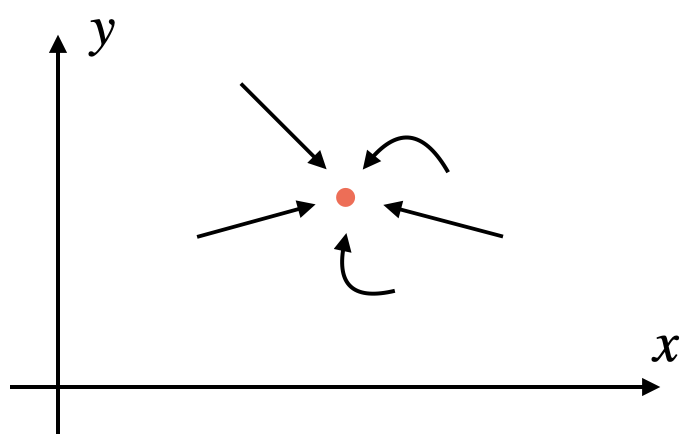
\includegraphics[width=45mm]{calculus10/limit2d.png}
 \end{center}
\end{figure}

\vspace{-3mm}

\end{frame}


%%%%%%%%%%%%%%%%%%%%%%%%%%%%%%%%%%%%%%%%%%%%%%%%%%%%%%%%%%%%%%%%%%%%%%%%%%%%%%%%%%%%%%%
%%%%%%%%%%%%%%%%%%%%%%%%%%%%%%%%%%%%%%%%%%%%%%%%%%%%%%%%%%%%%%%%%%%%%%%%%%%%%%%%%%%%%%%


\begin{frame}
\frametitle{極限が存在しない例}

$D=\{(x,y) \in \R^2 \ | \ (x,y) \ne (0,0)\}$で定義された関数$f(x,y)=\frac{x^2-y^2}{x^2+y^2}$を考える. 

\begin{itemize}
\item $y=0$を満たしながら$(x,y)$が$(0,0)$に近づく極限は
$$
\lim_{(x,0)\to (0,0)} \frac{x^2-y^2}{x^2+y^2} 
=\lim_{x\to 0} \frac{x^2}{x^2}  =\lim_{x\to 0} 1=1. 
$$
\item $x=0$を満たしながら$(x,y)$が$(0,0)$に近づく極限は
$$
\lim_{(0,y)\to (0,0)} \frac{x^2-y^2}{x^2+y^2} 
=\lim_{y\to 0} \frac{-y^2}{y^2}  =\lim_{x\to 0} -1=-1. 
$$
\end{itemize}
これより$\displaystyle \lim_{(x,y)\to (0,0)}f(x,y)$は存在しない. 
\end{frame}



%%%%%%%%%%%%%%%%%%%%%%%%%%%%%%%%%%%%%%%%%%%%%%%%%%%%%%%%%%%%%%%%%%%%%%%%%%%%%%%%%%%%%%%
%%%%%%%%%%%%%%%%%%%%%%%%%%%%%%%%%%%%%%%%%%%%%%%%%%%%%%%%%%%%%%%%%%%%%%%%%%%%%%%%%%%%%%%


\begin{frame}
\frametitle{極限が存在する例}

$D=\{(x,y) \in \R^2 \ | \ (x,y) \ne (0,0)\}$で定義された関数$f(x,y)=\frac{x^2y}{x^2+y^2}$について, $\displaystyle \lim_{(x,y)\to (0,0)}f(x,y)$を考察する. \\
\ \\

極座標$(r,\theta)$と呼ばれる
$$
x= r \cos \theta, \ \ \ y = r \sin \theta
$$
なる変数変換を考えると
$$
f(x,y)=\frac{(r\cos \theta)^2 r \sin \theta}{(r \cos \theta)^2+(r \sin \theta)^2}=r \cos^2 \theta \sin \theta. 
$$
$\sqrt{x^2+y^2}=r$に注意すると, $\displaystyle \lim_{(x,y)\to (0,0)}|f(x,y)|= \lim_{r \to 0} r=0$であるから, 
$$
\lim_{(x,y)\to (0,0)}f(x,y)=0.
$$
 
\end{frame}


%%%%%%%%%%%%%%%%%%%%%%%%%%%%%%%%%%%%%%%%%%%%%%%%%%%%%%%%%%%%%%%%%%%%%%%%%%%%%%%%%%%%%%%
%%%%%%%%%%%%%%%%%%%%%%%%%%%%%%%%%%%%%%%%%%%%%%%%%%%%%%%%%%%%%%%%%%%%%%%%%%%%%%%%%%%%%%%


\begin{frame}
\frametitle{連続性}


\begin{Def}
\begin{itemize}
\item 二変数関数$f(x,y)$がその定義域の点$(a,b)$で\underline{連続}であるとは
$$
\lim_{(x,y)\to (a,b)}f(x,y) = f(a,b)
$$
が成立すること. つまり左辺の極限が存在し, それが$f(a,b)$と一致すること. 
\item 定義域の任意の点で連続な関数を\underline{連続関数}という. 
\end{itemize}
\end{Def}

\end{frame}





%%%%%%%%%%%%%%%%%%%%%%%%%%%%%%%%%%%%%%%%%%%%%%%%%%%%%%%%%%%%%%%%%%%%%%%%%%%%%%%%%%%%%%%
%%%%%%%%%%%%%%%%%%%%%%%%%%%%%%%%%%%%%%%%%%%%%%%%%%%%%%%%%%%%%%%%%%%%%%%%%%%%%%%%%%%%%%%


%%%%%%%%%%%%%%%%%%%%%%%%%%%%%%%%%%%%%%%%%%%%%%%%%%%%%%%%%%%%%%%%%%%%%%%%%%%%%%%%%%%%%%%
%%%%%%%%%%%%%%%%%%%%%%%%%%%%%%%%%%%%%%%%%%%%%%%%%%%%%%%%%%%%%%%%%%%%%%%%%%%%%%%%%%%%%%%


\begin{frame}
\frametitle{連続性}

\begin{itemize}
\item 一変数関数の場合と同様に, 二変数関数も四則演算により連続性は保たれる. 
例えば, $f(x,y),g(x,y)$が$(a,b)$で連続であれば, 
$$
\alpha f(x,y)+\beta g(x,y), \ \ \ f(x,y)g(x,y) \ \ \ (\alpha,\beta \in \R)
$$
も$(a,b)$で連続. 
\item 特に変数$x,y$についての多項式関数, 有理式関数は連続関数.  
また連続性は合成によっても保たれ, これらと指数関数, 対数関数, 三角関数, 逆三角関数等を合成した関数も, その定義域において連続関数となる.  
\end{itemize}

\end{frame}



%%%%%%%%%%%%%%%%%%%%%%%%%%%%%%%%%%%%%%%%%%%%%%%%%%%%%%%%%%%%%%%%%%%%%%%%%%%%%%%%%%%%%%%
%%%%%%%%%%%%%%%%%%%%%%%%%%%%%%%%%%%%%%%%%%%%%%%%%%%%%%%%%%%%%%%%%%%%%%%%%%%%%%%%%%%%%%%


\section{偏微分(partial differential/differentiation)}


\begin{frame}
\frametitle{偏微分}

二変数関数は1つの変数以外を定数とみなして微分を考えることができる. 

\begin{Def}
二変数関数$f(x,y)$の変数$y$を定数$b$として, $x$のみを変数とする一変数関数$f(x,b)$が$x=a$で微分可能なとき, つまり極限
$$
\lim_{h \to 0} \frac{f(a+h,b)-f(a,b)}{h}
$$
が存在するとき, $f(x,y)$は$(a,b)$において$x$に関して\underline{偏微分可能}であるという. 
この極限を$f_x(a,b)$, $\frac{\partial f}{\partial x}(a,b)$などと書き, 
$f(x,y)$の$(a,b)$における$x$に関する\underline{偏微分係数}という. 
\end{Def}
$y$に関する偏微分可能性, 偏微分係数も同様に定める. 

\end{frame}



%%%%%%%%%%%%%%%%%%%%%%%%%%%%%%%%%%%%%%%%%%%%%%%%%%%%%%%%%%%%%%%%%%%%%%%%%%%%%%%%%%%%%%%
%%%%%%%%%%%%%%%%%%%%%%%%%%%%%%%%%%%%%%%%%%%%%%%%%%%%%%%%%%%%%%%%%%%%%%%%%%%%%%%%%%%%%%%


\begin{frame}
\frametitle{偏導関数}

\begin{Def}
二変数関数$f(x,y)$が定義域の任意の点において$x$に関して偏微分可能であるとき, $f(x,y)$は$x$に関して偏微分可能であるという. 
このとき関数$f_x(x,y)$または$\frac{\partial f}{\partial x}(x,y)$を$f(x,y)$の$x$に関する\underline{偏導関数}という. 
$x$に関する偏導関数を求めることを$x$に関して\underline{偏微分}するという. 
\end{Def}
$y$に関する偏導関数, 偏微分も同様に定める. 


\end{frame}


%%%%%%%%%%%%%%%%%%%%%%%%%%%%%%%%%%%%%%%%%%%%%%%%%%%%%%%%%%%%%%%%%%%%%%%%%%%%%%%%%%%%%%%
%%%%%%%%%%%%%%%%%%%%%%%%%%%%%%%%%%%%%%%%%%%%%%%%%%%%%%%%%%%%%%%%%%%%%%%%%%%%%%%%%%%%%%%


\begin{frame}
\frametitle{偏導関数}


二変数関数$f(x,y)=x^2y^3+4x-5y+6$の偏導関数を求める. 

\begin{itemize}
\item $x$を変数, $y$を定数とみなして, $x$に関する偏導関数を求める. 
\begin{align*}
f_x(x,y)=\frac{\partial}{\partial x}(x^2y^3+4x-5y+6) = 2xy^3+4. 
\end{align*}
\item $x$を定数, $y$を変数とみなして, $y$に関する偏導関数を求める. 
\begin{align*}
f_y(x,y)=\frac{\partial}{\partial y}(x^2y^3+4x-5y+6) = 3x^2y^2-5. 
\end{align*}
\end{itemize}

\begin{Prob}
$f(x,y)=xy^2+\sin x + \cos y$の偏導関数を求めよ. 
\end{Prob}

\end{frame}



%%%%%%%%%%%%%%%%%%%%%%%%%%%%%%%%%%%%%%%%%%%%%%%%%%%%%%%%%%%%%%%%%%%%%%%%%%%%%%%%%%%%%%%
%%%%%%%%%%%%%%%%%%%%%%%%%%%%%%%%%%%%%%%%%%%%%%%%%%%%%%%%%%%%%%%%%%%%%%%%%%%%%%%%%%%%%%%


\begin{frame}
\frametitle{偏導関数}

一変数関数は微分可能であれば連続であったが, 偏微分可能な二変数関数は連続とは限らない. 
例えば, $\R^2$で定義された
$$
f(x,y)=
\begin{cases}
\frac{xy}{x^2+y^2}  & ((x,y) \ne (0,0)) \\
0 & ((x,y)=(0,0)) 
 \end{cases}
$$
を考える. 
\begin{align*}
f_x(0,0) &=\lim_{h\to 0}\frac{f(0+h,0)-f(0,0)}{h}=\lim_{h\to 0}\frac{0-0}{h}=0, \\
f_y(0,0) &=\lim_{h\to 0}\frac{f(0,0+h)-f(0,0)}{h}=\lim_{h\to 0}\frac{0-0}{h}=0
\end{align*}
であるが, $\displaystyle \lim_{(x,x)\to (0,0)} f(x,y)= \frac{1}{2} \ne f(0,0)$\footnote{$x=y$の線に沿うと常に1/2}. 

\end{frame}



%%%%%%%%%%%%%%%%%%%%%%%%%%%%%%%%%%%%%%%%%%%%%%%%%%%%%%%%%%%%%%%%%%%%%%%%%%%%%%%%%%%%%%%
%%%%%%%%%%%%%%%%%%%%%%%%%%%%%%%%%%%%%%%%%%%%%%%%%%%%%%%%%%%%%%%%%%%%%%%%%%%%%%%%%%%%%%%


\begin{frame}
\frametitle{高次偏導関数}

\begin{Def}
二変数関数$f(x,y)$の偏導関数$f_x(x,y)$と$f_y(x,y)$がさらに$x$と$y$で偏微分可能であるとき, その偏導関数を$f(x,y)$の\underline{2次偏導関数}という. 
このとき$f(x,y)$は2回偏微分可能であるいう. 
\begin{itemize}
\item $f_x(x,y)$の$x$に関する偏導関数を
$$
f_{xx}(x,y)=\frac{\partial^2 f}{\partial x^2}(x,y)=\frac{\partial^2 f}{\partial x \partial x}(x,y)=\frac{\partial }{\partial x}\frac{\partial f}{\partial x}(x,y), 
$$
\item $f_x(x,y)$の$y$に関する偏導関数を
$$
f_{xy}(x,y)=\frac{\partial^2 f}{\partial y \partial x}(x,y)=\frac{\partial }{\partial y}\frac{\partial f}{\partial x}(x,y)
$$
\end{itemize}
などと表す. $f_y(x,y)$の偏微分も同様である. 
\end{Def}

\end{frame}



%%%%%%%%%%%%%%%%%%%%%%%%%%%%%%%%%%%%%%%%%%%%%%%%%%%%%%%%%%%%%%%%%%%%%%%%%%%%%%%%%%%%%%%
%%%%%%%%%%%%%%%%%%%%%%%%%%%%%%%%%%%%%%%%%%%%%%%%%%%%%%%%%%%%%%%%%%%%%%%%%%%%%%%%%%%%%%%


\begin{frame}
\frametitle{高次偏導関数}

\begin{itemize}
\item $f(x,y)$の$k$回偏微分可能性や$k$次偏導関数も同様に定義される. 
\item $k$次偏導関数は$2^k$通り考えられるが, 次の定理により, 多くの高次偏導関数は偏微分の順序に依存しない.  
\end{itemize}

\begin{Thm}
$f_{xy}(x,y)$と$f_{yx}(x,y)$が存在し, 連続であるとき$f_{xy}(x,y)=f_{yx}(x,y)$. 
\end{Thm}

\begin{itemize}
\item $f(x,y)$が$k$回偏微分可能で, $k$次までの全ての偏導関数が連続となるとき, $f(x,y)$は$k$回連続微分可能, または$C^k$級であるという. 
\item 無限回連続微分可能, $C^\infty$級も同様に定義される.
\end{itemize}
\end{frame}


%%%%%%%%%%%%%%%%%%%%%%%%%%%%%%%%%%%%%%%%%%%%%%%%%%%%%%%%%%%%%%%%%%%%%%%%%%%%%%%%%%%%%%%
%%%%%%%%%%%%%%%%%%%%%%%%%%%%%%%%%%%%%%%%%%%%%%%%%%%%%%%%%%%%%%%%%%%%%%%%%%%%%%%%%%%%%%%


\begin{frame}
\frametitle{高次偏導関数}

$f(x,y)=xy^2+\sin x + \cos y$の$2$次偏導関数を求める. 

\begin{itemize}
\item $f_x(x,y)=y^2+\cos x$
$$
f_{xx}(x,y)=-\sin x, \ \ \ f_{xy}(x,y)=2y. 
$$
\item $f_y(x,y)=2xy-\sin y$
$$
f_{yx}(x,y)=2y, \ \ \ f_{yy}(x,y)=2x-\cos y. 
$$
\end{itemize}
\end{frame}


%%%%%%%%%%%%%%%%%%%%%%%%%%%%%%%%%%%%%%%%%%%%%%%%%%%%%%%%%%%%%%%%%%%%%%%%%%%%%%%%%%%%%%%
%%%%%%%%%%%%%%%%%%%%%%%%%%%%%%%%%%%%%%%%%%%%%%%%%%%%%%%%%%%%%%%%%%%%%%%%%%%%%%%%%%%%%%%


\begin{frame}
\frametitle{高次偏導関数}

\begin{Prob}
次の関数の2次偏導関数を求めよ. 
\begin{enumerate}
\item $2x^3-3x^2y-4xy^2+5y^4$
\item $\frac{x}{y}$
\item $x \log y$
\item $x \cos(x+y)$
\end{enumerate}
\end{Prob}

\end{frame}

%%%%%%%%%%%%%%%%%%%%%%%%%%%%%%%%%%%%%%%%%%%%%%%%%%%%%%%%%%%%%%%%%%%%%%%%%%%%%%%%%%%%%%%
%%%%%%%%%%%%%%%%%%%%%%%%%%%%%%%%%%%%%%%%%%%%%%%%%%%%%%%%%%%%%%%%%%%%%%%%%%%%%%%%%%%%%%%


%\begin{frame}
%\frametitle{高次偏導関数}
%
%
%\begin{enumerate}
%\item $f_{xx}=12x-6y, f_{xy}=f_{yx}=-6x-8y, f_{yy}=-8x+60y^2$
%\item $f_{xx}=0, f_{xy}=f_{yx}=-\frac{1}{y^2}, f_{yy}=2\frac{x}{y^3}$
%\item $f_{xx}=0, f_{xy}=f_{yx}=\frac{1}{y}, f_{yy}=-\frac{x}{y^2}$
%\item $f_{xx}=-\cos(x+y)-\sin(x+y)-x\cos(x+y), f_{xy}=f_{yx}=-\sin(x+y)-x\cos(x+y), f_{yy}=-x\cos(x+y)$
%\end{enumerate}
%
%\end{frame}

%%%%%%%%%%%%%%%%%%%%%%%%%%%%%%%%%%%%%%%%%%%%%%%%%%%%%%%%%%%%%%%%%%%%%%%%%%%%%%%%%%%%%%%
%%%%%%%%%%%%%%%%%%%%%%%%%%%%%%%%%%%%%%%%%%%%%%%%%%%%%%%%%%%%%%%%%%%%%%%%%%%%%%%%%%%%%%%


%\begin{frame}
%\frametitle{全微分(total differential/differentiation)}
%
%偏微分は一変数関数の微分を用いて簡単に定義することができるが, 極限の取り方が限られているため, 不都合なことが多い. 
%そこで一変数関数の微分を全微分と呼ばれる概念へ一般化する. 
%
%\begin{Def}
%二変数関数$f(x,y)$が$(a,b)$で\underline{全微分可能}であるとは, ある$A, B \in \R$が存在して
%$$
%\lim_{(h,k)\to0}\frac{f(a+h,b+k)-f(a,b)-Ah-Bk}{\sqrt{h^2+k^2}}=0
%$$
%が成立すること. 
%\end{Def}
%
%$f(x,y)$が$(a,b)$で全微分可能であるとき, $(a,b)$で連続かつ偏微分可能であり, 
%$$
%A=f_x(a,b), \ \ \ B=f_y(a,b). 
%$$
%\end{frame}
%

%%%%%%%%%%%%%%%%%%%%%%%%%%%%%%%%%%%%%%%%%%%%%%%%%%%%%%%%%%%%%%%%%%%%%%%%%%%%%%%%%%%%%%%
%%%%%%%%%%%%%%%%%%%%%%%%%%%%%%%%%%%%%%%%%%%%%%%%%%%%%%%%%%%%%%%%%%%%%%%%%%%%%%%%%%%%%%%


%\begin{frame}
%\frametitle{全微分}
%
%\begin{itemize}
%\item 一変数関数に関しては, 微分可能性は一次式で近似できる(接線が存在する)と同値であった. 
%\item 二変数関数に関しては, $x, y$で偏微分可能であっても一次式で近似できる(接平面が存在する)とは限らない. 
%\item 二変数関数$f(x,y)$が$(a, b)$で全微分可能であれば, そのグラフの接平面を与える一次式
%$$
%z=f(a,b)+f_x(a,b)(x-a)+f_y(a,b)(y-b)
%$$
%で$f(x,y)$は$(a, b)$の近傍で近似される. 
%\end{itemize}
%
%\end{frame}



%%%%%%%%%%%%%%%%%%%%%%%%%%%%%%%%%%%%%%%%%%%%%%%%%%%%%%%%%%%%%%%%%%%%%%%%%%%%%%%%%%%%%%%
%%%%%%%%%%%%%%%%%%%%%%%%%%%%%%%%%%%%%%%%%%%%%%%%%%%%%%%%%%%%%%%%%%%%%%%%%%%%%%%%%%%%%%%


%\begin{frame}
%\frametitle{全微分可能性}
%
%\begin{Thm}
%$f(x,y)$が$C^1$級(各成分について偏微分可能, かつ偏導関数が連続)であれば, 全微分可能である. 
%\end{Thm}
%
%例えば, $\R^2$で定義された
%$$
%f(x,y)=
%\begin{cases}
%\frac{x|y|}{\sqrt{x^2+y^2}}  & ((x,y) \ne (0,0)) \\
%0 & ((x,y)=(0,0)) 
% \end{cases}
%$$
%は原点において全微分不可能である(偏微分可能であるが, 偏導関数は連続でない).  
%実際の計算に現れる関数は$C^\infty$級であることが多いので, あまり神経質になる必要はない.
%
%\end{frame}


%%%%%%%%%%%%%%%%%%%%%%%%%%%%%%%%%%%%%%%%%%%%%%%%%%%%%%%%%%%%%%%%%%%%%%%%%%%%%%%%%%%%%%%
%%%%%%%%%%%%%%%%%%%%%%%%%%%%%%%%%%%%%%%%%%%%%%%%%%%%%%%%%%%%%%%%%%%%%%%%%%%%%%%%%%%%%%%


\begin{frame}
\frametitle{接平面}

二変数関数$f(x,y)=x^2+3y^2$のグラフの点$(1,2,13)$における接平面を求める. 
$$
f_x(x,y)=2x=2, \ \ \ f_y(x,y)=6y=12
$$
より, $f(x,y)$は$C^1$級であるから, 接平面の方程式は
$$
z=13+2(x-1)+12(y-2)
$$
で与えられる. 整理すれば
$$
z=2x+12y-13. 
$$

\end{frame}


%%%%%%%%%%%%%%%%%%%%%%%%%%%%%%%%%%%%%%%%%%%%%%%%%%%%%%%%%%%%%%%%%%%%%%%%%%%%%%%%%%%%%%%
%%%%%%%%%%%%%%%%%%%%%%%%%%%%%%%%%%%%%%%%%%%%%%%%%%%%%%%%%%%%%%%%%%%%%%%%%%%%%%%%%%%%%%%


\begin{frame}
\frametitle{極値と停留点}

以下では, 二変数関数$f(x,y)$は$C^2$級であるとする. 
$f(x,y)$の\underline{停留点}とは, $f_x(a,b) = f_y(a,b) = 0$を満たす$(a,b)$をいう. 

\begin{Thm} \label{極値->停留点}
関数$f(x,y)$が$(a,b)$で極値(極大値または極小値)を取るとき, $(a,b)$は停留点となる. 
\end{Thm}

\begin{itemize}
\item 定理\ref{極値->停留点}は, 一変数関数$f(x,b)$と$f(a,y)$が$(a,b)$で極値を取ることから従う. 
\item 停留点は極値とは限らない. 例えば, \underline{鞍点(あんてん:saddle point)}と呼ばれる, ある方向から見ると極大値, 別の方向から見ると極小値となる停留点も存在する. 
\end{itemize}

\end{frame}




%%%%%%%%%%%%%%%%%%%%%%%%%%%%%%%%%%%%%%%%%%%%%%%%%%%%%%%%%%%%%%%%%%%%%%%%%%%%%%%%%%%%%%%
%%%%%%%%%%%%%%%%%%%%%%%%%%%%%%%%%%%%%%%%%%%%%%%%%%%%%%%%%%%%%%%%%%%%%%%%%%%%%%%%%%%%%%%


\begin{frame}
\frametitle{極値問題の主定理}


\begin{Thm} \label{停留点とヘッセ行列}
関数$f(x,y)$の\underline{ヘッセ行列式}(ヘッシアン)を
$$
H(x,y)
=f_{xx}(x,y)f_{yy}(x,y)-f_{xy}(x,y)^2
$$
で定義する. 
停留点$(a,b)$に関して 
\begin{itemize}
\item $H(a,b)>0, \ f_{xx}(a,b)>0 \ \Longrightarrow$ $f(x,y)$は$(a,b)$で極小, 
\item $H(a,b)>0, \ f_{xx}(a,b)<0 \ \Longrightarrow$ $f(x,y)$は$(a,b)$で極大, 
\item $H(a,b)<0 \ \Longrightarrow$ $(a,b)$は$f(x,y)$の鞍点. 
\end{itemize}
\end{Thm}

%$H(a,b)>0$の下で, 条件$f_{xx}(a,b) \gtrless 0$は条件$f_{yy}(a,b)\gtrless 0$と同値であることに注意する. 
証明は後述。
\end{frame}



%%%%%%%%%%%%%%%%%%%%%%%%%%%%%%%%%%%%%%%%%%%%%%%%%%%%%%%%%%%%%%%%%%%%%%%%%%%%%%%%%%%%%%%
%%%%%%%%%%%%%%%%%%%%%%%%%%%%%%%%%%%%%%%%%%%%%%%%%%%%%%%%%%%%%%%%%%%%%%%%%%%%%%%%%%%%%%%


\begin{frame}
\frametitle{極値問題}

関数$f(x,y)=x^2+x^2y+y^2$の極値を調べる. まず
\begin{align*}
f_x(x,y) &= 2x+2xy=2x(1+y)=0\\ 
f_y(x,y) &= x^2+2y=0
\end{align*}
を解くことで, 停留点は
$$
(x,y)=(0,0), \ (\pm \sqrt{2},-1)
$$
だと分かる. 

\end{frame}


%%%%%%%%%%%%%%%%%%%%%%%%%%%%%%%%%%%%%%%%%%%%%%%%%%%%%%%%%%%%%%%%%%%%%%%%%%%%%%%%%%%%%%%
%%%%%%%%%%%%%%%%%%%%%%%%%%%%%%%%%%%%%%%%%%%%%%%%%%%%%%%%%%%%%%%%%%%%%%%%%%%%%%%%%%%%%%%


\begin{frame}
\frametitle{極値問題}
また2次偏導関数は
$$
f_{xx}(x,y)=2(1+y), \ \ \ f_{xy}(x,y)=2x, \ \ \ f_{yy}(x,y)=2
$$
であるから
$$
H(x,y)=2(1+y) \cdot 2 - (2x)^2=4(1+y-x^2). 
$$

\begin{itemize}
\item 点$(0,0)$に関して
\begin{align*}
H(0,0)=4>0, \ \ \ f_{xx}(0,0) = 2
\end{align*}
であるから, $f(x,y)$は $f(0,0)=0$において極小値である. 
\item 点$(\pm \sqrt{2},-1)$に関して
\begin{align*}
H(\pm \sqrt{2},-1)=-8<0
\end{align*}
であるから, $f(x,y)$は$(\pm\sqrt{2},-1)$において極値をとらない.  
\end{itemize}

\end{frame}
\begin{slide}{$f(x,y) = x^2+x^2y+y^2$のグラフ}
\begin{figure}[h]
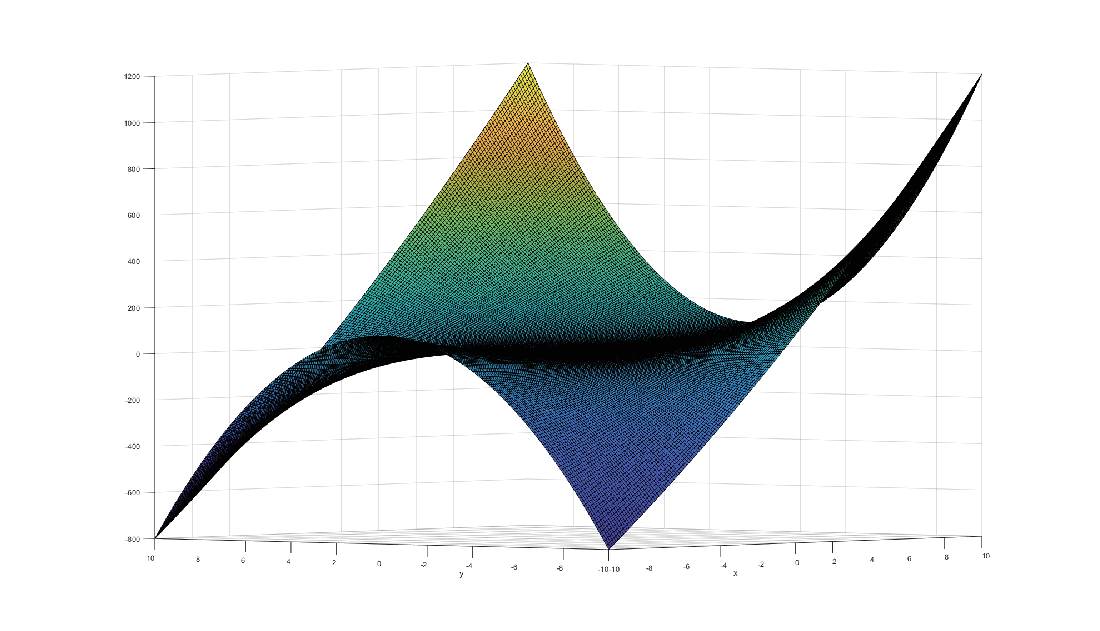
\includegraphics[width=8cm]{calculus10/twodimopt.eps}
\end{figure}
twodimopt.m参照。
\end{slide}


%%%%%%%%%%%%%%%%%%%%%%%%%%%%%%%%%%%%%%%%%%%%%%%%%%%%%%%%%%%%%%%%%%%%%%%%%%%%%%%%%%%%%%%
%%%%%%%%%%%%%%%%%%%%%%%%%%%%%%%%%%%%%%%%%%%%%%%%%%%%%%%%%%%%%%%%%%%%%%%%%%%%%%%%%%%%%%%
\begin{slide}{二変数関数のテイラー展開}

二変数のテイラー展開は以下である。
\begin{eqnarray}
f(x+h, y+k) &=& f + \left(h\frac{\partial }{\partial x} + k\frac{\partial}{\partial y}\right) f \nonumber \\ 
&+& \frac{1}{2!}\left(h\frac{\partial }{\partial x} + k\frac{\partial}{\partial y}\right) ^2 f  \nonumber \\
&+& \frac{1}{3!}\left(h\frac{\partial }{\partial x} + k\frac{\partial}{\partial y}\right) ^3f + \cdots \nonumber
\end{eqnarray}

二次まで展開すると
\begin{eqnarray}
&& f(x+h, y+k) =  f + \left(h\frac{\partial f}{\partial x} + k\frac{\partial f}{\partial y}\right)  \nonumber \\ 
&+& \frac{1}{2!}\left(h^2\frac{\partial^2 f}{\partial x^2} + 2hk\frac{\partial^2 f}{\partial x\partial y}+k^2\frac{\partial^2 f}{\partial y^2}\right)  \nonumber \\
&=& f + hf_x + kf_y + \frac{h^2}{2}f_{xx}+ hk f_{xy} + \frac{k^2}{2}f_{yy} \nonumber
\end{eqnarray}

\end{slide}

%\begin{frame}
%\frametitle{極値と停留点 (発展)}
%
%二変数関数に関しても, テイラー展開を行うことが可能で
%$C^2$級関数$f(x,y)$は停留点$(a,b)$の近傍で次の形に近似される. 
%(停留点という条件から, 一次部分は消えている.)
%\begin{align*}
%f(x,y) & \approx f(a,b)+ \frac{1}{2}f_{xx}(a,b)(x-a)^2 \\
%& \ \ \ \ \ \ +f_{xy}(a,b)(x-a)(y-b)+\frac{1}{2}f_{yy}(a,b)(y-b)^2 \\
%& =  f(a,b)+ \frac{1}{2}[x-a \ \ y-b]
%\begin{bmatrix} f_{xx}(a,b) & f_{xy}(a,b) \\ f_{yx}(a,b) & f_{yy}(a,b) \end{bmatrix}
%\begin{bmatrix} x-a \\ y-b \end{bmatrix}
%\end{align*}
%ヘッセ行列式$H(a,b)$は$\begin{bmatrix} f_{xx}(a,b) & f_{xy}(a,b) \\ f_{yx}(a,b) & f_{yy}(a,b) \end{bmatrix}$の行列式に他ならない. 
%定理\ref{停留点とヘッセ行列}は対称2次形式の分類に関係する. 
%
%\end{frame}

\begin{slide}{極大・極小の判別原理}
$x,y$の二次斉次式(せいじしき:すべての項の次数が等しい式:homogeneous polynomial)$Q(x) = Ax^2 + 2Bxy+ Cy^2$は
\begin{enumerate}
\item $AC-B^2>0, A>0$なら$(0,0)$で極小
\item $AC-B^2>0, A<0$なら$(0,0)$で極大
\item $AC-B^2<0$なら極大・極小をとらない
\end{enumerate}
証明
\begin{equation}
Q(x,y) = A\left\{\left(x + \frac{B}{A}y\right)^2 + \frac{AC-B^2}{A^2}y^2\right\}\nonumber 
\end{equation}
と変形でき$(x + \frac{B}{A}y)^2$は常に正、$AC-B^2$が正で、$A>0$の時$Q>0$(極小), $A<0$の時$Q<0$(極大)となる。
$AC-B^2$が負の場合には、$Q$は正にも負にもなる。

これを利用し、関数$f$の二次までのテイラー展開は
\begin{equation}
f(x+h, y+k) = f(x,y) + f_x(x,y)h + f_y(x,y)k + f_{xy}(x,y)kh + \frac{f_{xx}}{2}h^2 + \frac{f_{yy}}{2}k^2 \nonumber
\end{equation}
であり、極値では$f_x(x,y)=f_y(x,y)=0$であり、斉次式を適用。
\end{slide}

%%%%%%%%%%%%%%%%%%%%%%%%%%%%%%%%%%%%%%%%%%%%%%%%%%%%%%%%%%%%%%%%%%%%%%%%%%%%%%%%%%%%%%%
%%%%%%%%%%%%%%%%%%%%%%%%%%%%%%%%%%%%%%%%%%%%%%%%%%%%%%%%%%%%%%%%%%%%%%%%%%%%%%%%%%%%%%%





%%%%%%%%%%%%%%%%%%%%%%%%%%%%%%%%%%%%%%%%%%%%%%%%%%%%%%%%%%%%%%%%%%%%%%%%%%%%%%%%%%%%%%%
%%%%%%%%%%%%%%%%%%%%%%%%%%%%%%%%%%%%%%%%%%%%%%%%%%%%%%%%%%%%%%%%%%%%%%%%%%%%%%%%%%%%%%%


%\begin{slide}{課題\#10}
%関数$f (x, y) = xy(1 - x - y) $の極値を求め、それぞれが極大か極小を判別せよ. 
%
%\end{slide}

\begin{slide}{課題\#10}
ある地域の家賃$y$万円と、部屋の広さ$x$~$\mathrm{m^2}$のデータを集めて、相場を推定する仕事を担当したとしよう。$i$番目の家賃と、部屋の広さのデータを$y_i, x_i$で表して、データが下のように$15$個集められたとする。
\begin{table}[hbt]
\centering 
%\caption{部屋の広さと家賃に関するデータ}
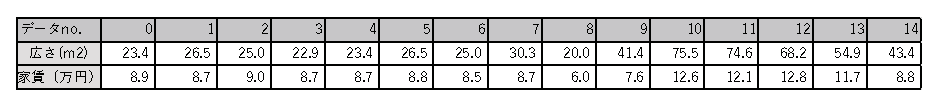
\includegraphics[width=10cm]{calculus10/renttab.eps}
\label{tab:renttab}
\end{table}
このデータを用いて部屋の広さ$x$を与えると家賃相場$y$がある定数$a, b$を用いて
\begin{equation}
y = a x + b \nonumber
\label{eq:regsimple}
\end{equation}
で計算できるようにしたい。$a,b$をデータ$(x_0, y_0), (x_1, y_1), \cdots, (x_{14}, y_{14})$を用いて、以下の損失関数$L(a,b)$を最小にするように選ぶ場合、
\begin{equation}
L(a, b) = \sum_{i=0}^{14} \left(a x_i + b - y_i\right)^2 \nonumber 
\end{equation}
$a, b$はいくつになるか?導出経緯も説明しなさい。




\end{slide}

\section{今日のまとめ}
\begin{frame}
\frametitle{まとめ}   


\begin{enumerate}
\item 二変数関数, 極限, 連続性
\item 偏微分, 高次偏導関数,
\item 接平面, 極値問題, ヘッセ行列式
\end{enumerate} 

\end{frame}
